\chapter{Mikroba dan Infeksi}\label{ch:g9:microbes-and-infection}

Mereka sudah membayangi buku ini sejak \omterm{def:g1:healthy-habits:germs}{kuman} yang tak
terlihat pada tahun pertama
(\cref{def:g1:healthy-habits:germs}): naik menjadi tenaga
kerja di toko rotinya (\cref{ch:g6:producing-our-food}),
menjadi regu \omterm{def:g6:decomposers-and-soil:decomposers}{pengurai} di dalam \omterm{def:g6:decomposers-and-soil:soil}{tanahnya}, menjadi lawan yang
berevolusi di bangsal rumah sakitnya
(\cref{ex:g9:how-species-change:resistance}). Bab ini
akhirnya memberi \omterm{def:g6:producing-our-food:fermentation}{mikrobanya} laporan lengkapnya: mereka itu
apa, bagaimana minoritas yang merugikan menyerang, dan
bagaimana pertahanan luar tubuhnya --- dan pertahanan kita
--- menahan pintunya.

\section{Dunia mikrobanya}

\begin{definition}[Mikroba, dipilah]\label{def:g9:microbes-and-infection:sorted}
Yang disebut \emph{mikroorganisme}\index{mikroorganisme} ---
\omterm{def:g6:producing-our-food:fermentation}{mikroba} --- adalah \omterm{def:g6:exploring-our-environment:components}{makhluk hidup} yang terlalu kecil untuk
dilihat tanpa alat bantu. Jenis utamanya:
\begin{itemize}
  \item \emph{bakteri}\index{bakteri}: \omterm{def:g5:first-look-at-cells:cell}{sel} tunggal tanpa
        \omterm{def:g6:cell-unit-of-life:parts}{inti sel} sejati, jauh lebih kecil daripada selmu,
        membelah dengan cepat (dunia pada
        \cref{def:g6:cell-unit-of-life:unicellular}) --- ada
        di mana-mana, dalam jumlah yang tak terhitung;
  \item \emph{fungi \omterm{def:g6:cell-unit-of-life:unicellular}{bersel tunggal} dan yang lain}: \omterm{ex:g6:producing-our-food:bread}{ragi}
        (\cref{ex:g6:producing-our-food:bread}), \omterm{def:g4:plants-without-seeds:spore}{spora}
        kapang, perenang setetes air kolamnya;
  \item \emph{virus}\index{virus}: lebih kecil lagi, dan
        berbeda jenisnya --- sepotong teks genetik yang
        dikemas (huruf pada \cref{def:g9:genes-and-dna:dna})
        di dalam sebuah mantel, \emph{tanpa \omterm{def:g5:first-look-at-cells:cell}{sel} dan tanpa
        kehidupannya sendiri}: sebuah virus tidak melakukan
        apa pun sampai ia masuk ke dalam sebuah \omterm{def:g5:first-look-at-cells:cell}{sel} hidup
        lalu memalingkan permesinan pembacaan \omterm{def:g5:first-look-at-cells:cell}{sel} itu untuk
        menyalin teks sang penyusup. Pada tanda
        \cref{prop:g1:living-or-not:signs}, virus duduk
        persis di tepi kehidupannya.
\end{itemize}
\end{definition}

\begin{proposition}[Sebagian besar tak merugikan, sering justru penting]\label{prop:g9:microbes-and-infection:mostly}
Nama buruknya adalah laporan minoritas. Sebagian besar
\omterm{def:g6:producing-our-food:fermentation}{mikroba} mengabaikan kita; banyak yang melayani kita: regu
\omterm{prop:g6:decomposers-and-soil:decomposition}{penguraiannya}
(\cref{def:g6:decomposers-and-soil:decomposers}), tenaga
kerja pangannya, ahli kimia \omterm{def:g6:decomposers-and-soil:soil}{tanahnya} --- dan \emph{flora
penetap}\index{flora penetap} yang tinggal di tubuhmu
sendiri: triliunan \omterm{def:g9:microbes-and-infection:sorted}{bakteri} tak merugikan yang menghamparkan
diri di \omterm{def:g1:the-five-senses:sense}{kulit} dan ususmu, membantu \omterm{def:g4:journey-of-food:digestion}{pencernaannya} dan,
\omterm{def:g1:the-five-senses:sense}{semata-mata} dengan menduduki tempatnya, mendesak penyusupnya
turun dari lahannya. Hanya minoritas yang kecil --- yaitu
\emph{patogen}\index{patogen} --- yang menyebabkan penyakit.
\end{proposition}
\admitted

\begin{example}[Satu tubuh, tiga hubungan]\label{ex:g9:microbes-and-infection:relations}
Di kulitmu menit ini: penetap bermiliar-miliar, yang menahan
permukaannya (hubungan satu: persekutuan). Di dalam yoghurt
sarapanmu: pekerja, yang mengasamkan atas perintah (hubungan
dua: pekerjaan, \cref{ex:g6:producing-our-food:yogurt}).
Pada paku berkarat di gudangnya: \omterm{def:g4:plants-without-seeds:spore}{spora} \omterm{def:g9:microbes-and-infection:sorted}{bakteri} rahang
terkunci, yang menunggu sebuah luka yang dalam (hubungan
tiga: minoritas \omterm{prop:g9:microbes-and-infection:mostly}{patogennya}, dan alasan bagi
\cref{ch:g9:immune-defenses} serta suntikan ulang
tetanusnya).
\end{example}

\section{Infeksi: serangannya, bertahap}

\begin{definition}[Tahap infeksinya]\label{def:g9:microbes-and-infection:stages}
Yang disebut \emph{infeksi}\index{infeksi} berjalan dalam
beberapa tahap, masing-masing dengan namanya:
\begin{enumerate}
  \item \emph{penularannya}: \omterm{prop:g9:microbes-and-infection:mostly}{patogennya} berjalan ---
        permukaan yang tersentuh dan tangan, tetesan yang
        terbatukkan, makanan dan air yang tercemar, \omterm{prop:g4:journey-of-food:absorb}{darah},
        dan jalur seksual yang ditandai
        \cref{def:g8:contraception:condom};
  \item \emph{masuknya}: lewat sebuah bobolan --- \omterm{def:g1:the-five-senses:sense}{kulit} yang
        tersayat, atau pintu tubuh yang terbuka: saluran
        napas, usus, dan jalur di atasnya;
  \item \emph{perbanyakannya}: hangat, basah dan disuapi,
        yang tiba itu membelah --- \omterm{def:g9:microbes-and-infection:sorted}{bakterinya} menurut aturan
        \omterm{def:g6:exploring-our-environment:conditions}{kondisi} pada \cref{prop:g6:decomposers-and-soil:speed},
        dan jumlahnya berlipat dua dalam hitungan jam;
        \omterm{def:g9:microbes-and-infection:sorted}{virusnya} dengan mengubah \omterm{def:g5:first-look-at-cells:cell}{sel} menjadi toko fotokopi;
  \item \emph{penyakitnya}: gejalanya --- dari kerusakannya
        sendiri, dari racun \omterm{def:g9:microbes-and-infection:sorted}{bakterinya}, dan sebagian (bab
        berikutnya) dari pertempuran pertahanannya sendiri.
\end{enumerate}
\end{definition}

\begin{example}[Dua penyusup, dipertentangkan]\label{ex:g9:microbes-and-infection:contrast}
\omterm{def:g9:microbes-and-infection:sorted}{Bakteri} luka sayatnya melawan \omterm{def:g9:microbes-and-infection:sorted}{virus} pilek musim dinginnya.
\omterm{def:g9:microbes-and-infection:sorted}{Bakterinya}: masuk lewat bobolannya, memperbanyak diri
\emph{di antara} \omterm{def:g5:first-look-at-cells:cell}{sel} di dalam jaringan yang hangat dan
basah, dan buangannya meracuni tetangganya --- denyut nyeri
dan nanah pada jari yang bernanah. \omterm{def:g9:microbes-and-infection:sorted}{Virusnya}: menumpang
sebuah tetesan sampai ke lapisan saluran napasnya, masuk ke
dalam \omterm{def:g5:first-look-at-cells:cell}{sel} lapisan itu sendiri, dan tiap \omterm{def:g5:first-look-at-cells:cell}{sel} yang dibajaknya
melepaskan segerombol salinan sebelum tumbang --- tenggorokan
yang perih dan hidung yang meler di sepanjang jejaknya.
Mekanika yang berbeda; antibiotik yang melaparkan yang
pertama tak dapat menyentuh yang kedua, sebab yang kedua
meminjam permesinan \emph{milikmu}, dan obat terhadapnya
sukar dibidikkan.
\end{example}

\section{Menahan pintunya}

\begin{proposition}[Pertahanan pertamanya]\label{prop:g9:microbes-and-infection:doors}
Sebelum pertempuran apa pun, tubuhnya menahan perbatasannya:
\begin{itemize}
  \item \emph{\omterm{def:g1:the-five-senses:sense}{kulit}}: kering, berlapis, memperbarui diri ---
        dindingnya (organ pada
        \cref{def:g1:the-five-senses:sense}, bertugas jaga);
  \item \emph{lapisan dalam dan sapunya}: permukaan
        pembersih saluran napasnya
        (\cref{prop:g7:lungs-and-gas-exchange:smoke}
        memperlihatkannya kewalahan), kimia pembilas air
        \omterm{def:g1:the-five-senses:sense}{mata} dan \omterm{def:g4:journey-of-food:tract}{air liurnya}, rendaman asam \omterm{def:g4:journey-of-food:tract}{lambungnya}
        (\cref{pb:g7:digestion-and-nutrients:1} mensterilkan
        sambil mencerna);
  \item \emph{para penetapnya}: lahan yang sudah diduduki
        floranya, sedikit ruang untuk pendaratan;
\end{itemize}
dan \omterm{def:g1:healthy-habits:hygiene}{kebersihan diri} memperpanjangnya: sabun pada
\cref{met:g1:healthy-habits:hands} (kini dengan mekanisme
lengkapnya --- penularannya diputus), air yang aman,
makanan yang dimasak dan disimpan dingin (penolakan \omterm{def:g6:exploring-our-environment:conditions}{kondisi}
pada \cref{rem:g6:producing-our-food:goodbad}), jarum yang
disterilkan, penghadang \omterm{def:g8:contraception:condom}{kondomnya}. Setiap aturan \omterm{def:g1:healthy-habits:hygiene}{kebersihan diri}
pada buku ini adalah sebuah tahap penularan atau masuknya,
yang dihadang.
\end{proposition}
\admitted

\begin{omfigure}
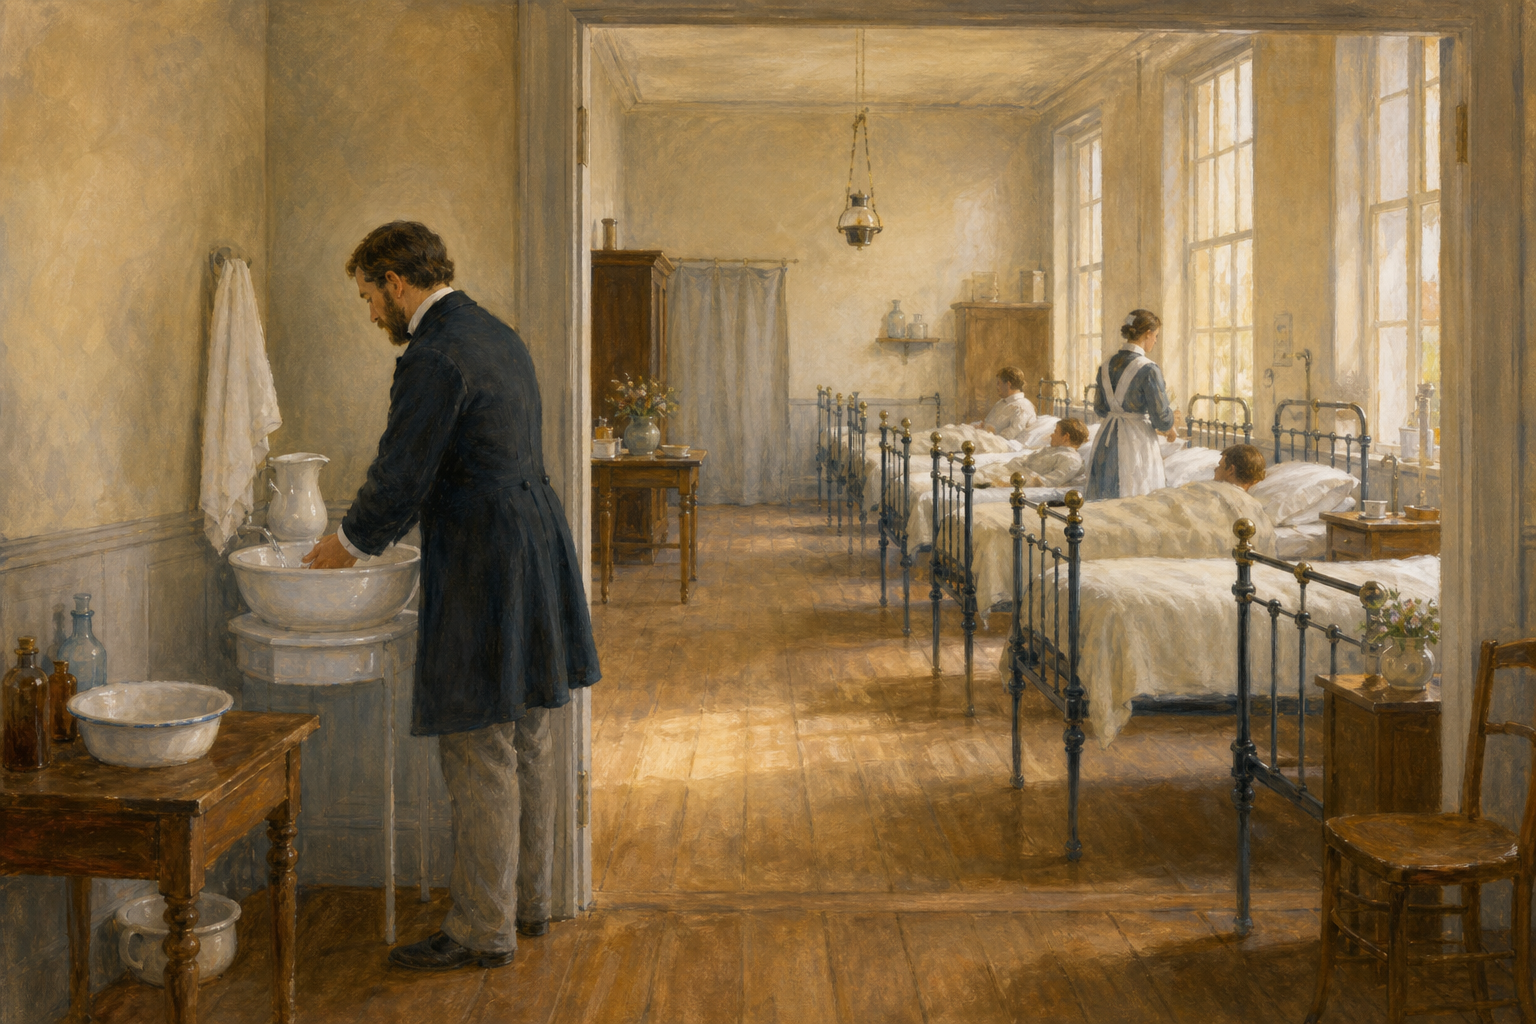
\includegraphics[width=0.6\linewidth]{images/book1/ai/g9-microbe-washing.png}

{\small Obat termurah dalam sejarah: sebuah baskom di pintu
bangsalnya, yang memutus kurir yang tak terlihat \omterm{def:g1:the-five-senses:sense}{mata}.}
\end{omfigure}

\begin{example}[Dua dokter yang menggerakkan angkanya]\label{ex:g9:microbes-and-infection:history}
Dua nama menambatkan sejarahnya. Semmelweis, Wina tahun
1840-an: kematian akibat demam nifas ambruk di bangsal
bersalinnya ketika para dokter mencuci tangan antara ruang
bedah mayat dan ruang bersalinnya --- penularannya diputus
sebelum seorang pun melihat sang pengembara. Pasteur, satu
angkatan kemudian, memperlihatkan para pengembaranya
sendiri: \omterm{def:g6:producing-our-food:fermentation}{mikroba}, bukan ``udara buruk'', yang mengasamkan
anggurnya, membunuh \omterm{ex:g2:animals-grow-up:butterfly}{ulat} suteranya, menulari lukanya ---
dan panas (\emph{pasteurisasi} temuannya) atau sterilisasi
yang menghentikannya. Teori \omterm{def:g1:healthy-habits:germs}{kuman} mengubah rumah sakit dari
bahaya menjadi pertahanan dalam satu masa hidup.
\end{example}

\begin{omfigure}
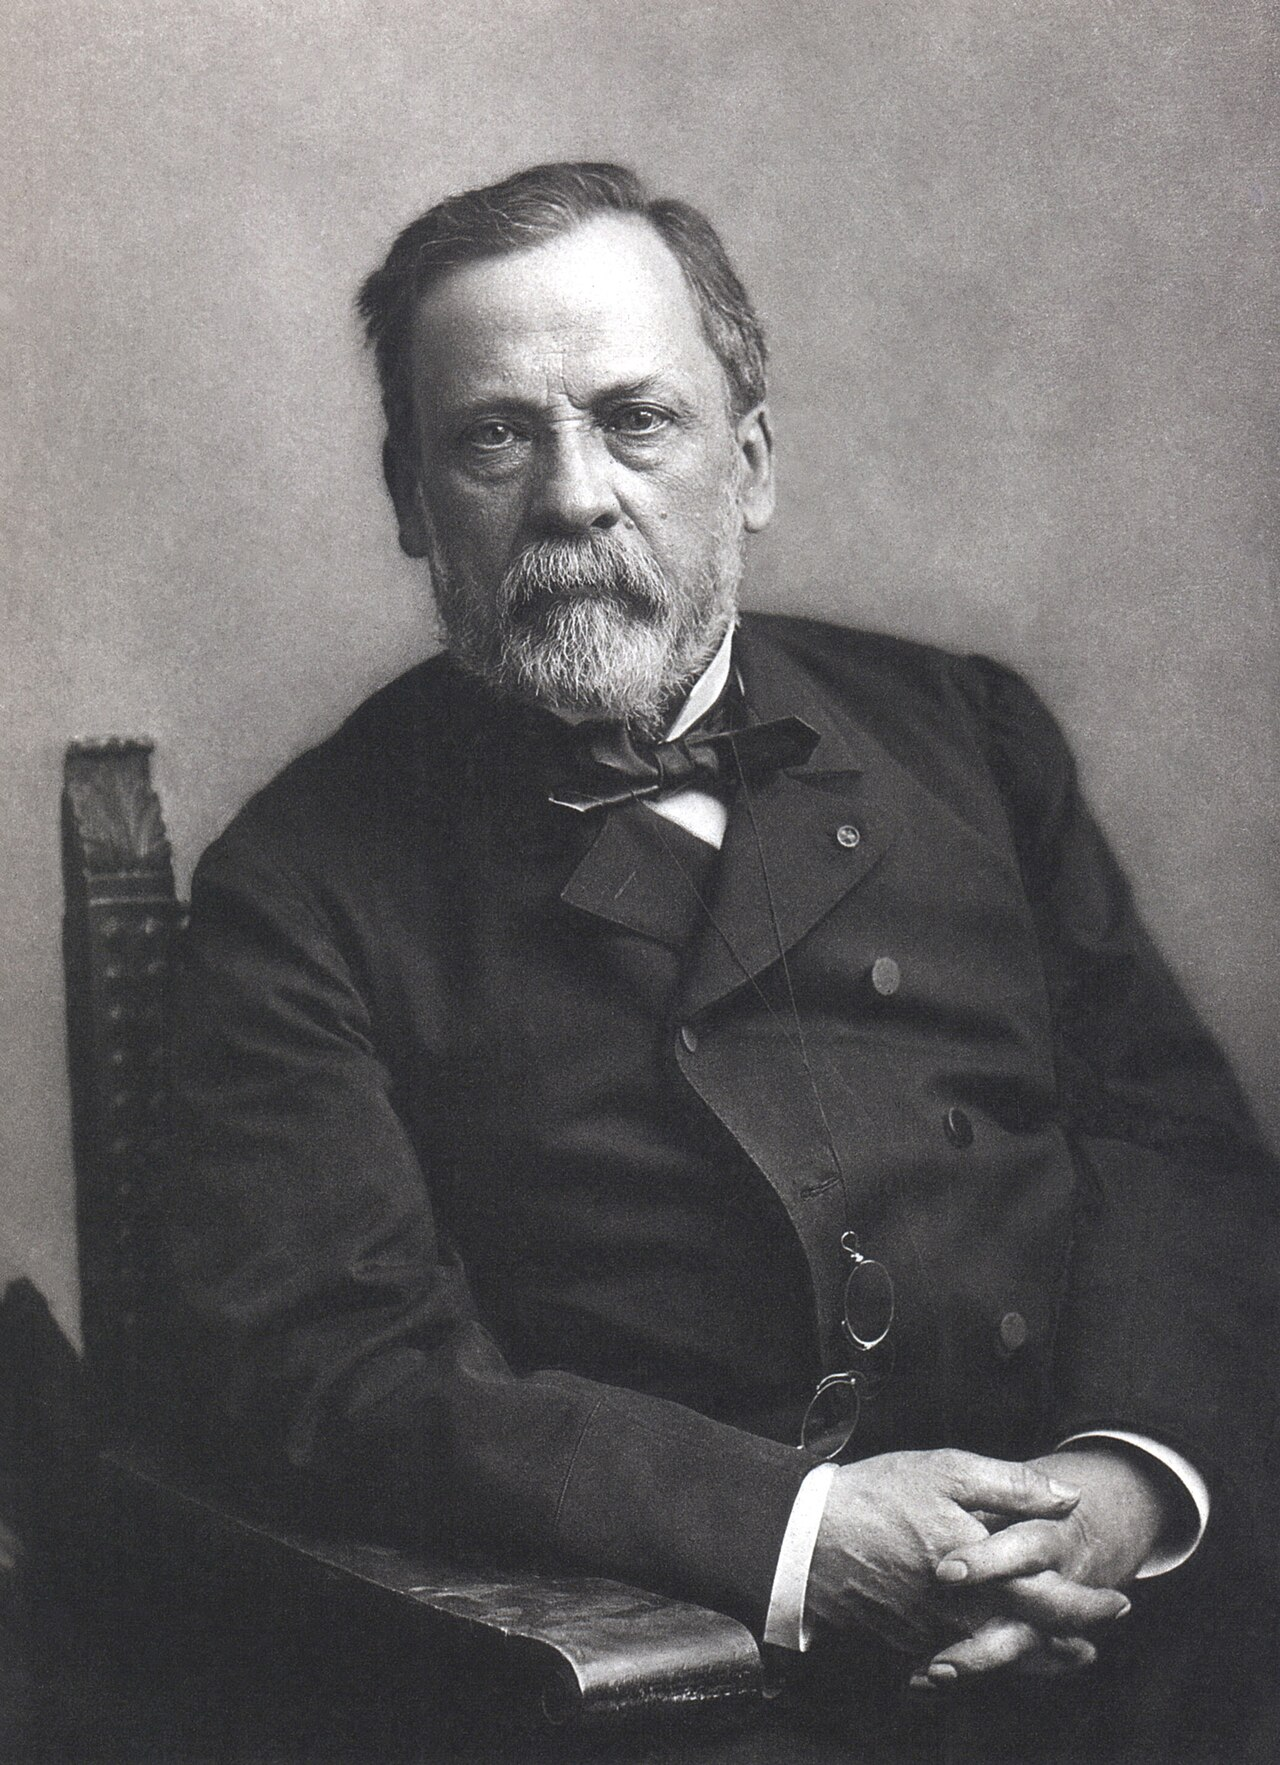
\includegraphics[width=0.42\linewidth]{images/book1/pasteur.jpg}

{\small Louis Pasteur, difoto oleh Paul Nadar: ilmuwan yang
memperlihatkan para pengembara tak terlihatnya sendiri.}
\end{omfigure}

\begin{method}[Mengaudit sebuah risiko infeksi]\label{met:g9:microbes-and-infection:audit}
Untuk keadaan apa pun --- dapur, luka, bangsal, kerumunan:
\begin{enumerate}
  \item sebutkan \omterm{prop:g9:microbes-and-infection:mostly}{patogen} yang masuk akal beserta jenisnya
        (\omterm{def:g9:microbes-and-infection:sorted}{bakteri}, \omterm{def:g9:microbes-and-infection:sorted}{virus}, fungi);
  \item telusuri jalur penularannya kepadamu;
  \item temukan pintu masuknya;
  \item tanyakan apa yang memperbanyaknya --- kehangatan,
        \omterm{def:g6:exploring-our-environment:conditions}{kelembapan}, makanan, waktu;
  \item hadanglah tahap yang paling murah: cuci, masak,
        tutup, dinginkan, sterilkan, vaksinasi
        (\cref{ch:g9:immune-defenses} menjelaskan yang
        terakhir).
\end{enumerate}
\end{method}

\section{Latihan}

\begin{exercise}[$\star$]\label{exo:g9:microbes-and-infection:1}
Sebutkan jenis \omterm{def:g6:producing-our-food:fermentation}{mikroba} utamanya, dan apa yang membedakan \omterm{def:g9:microbes-and-infection:sorted}{virus}.
\end{exercise}

\begin{exercise}[$\star$]\label{exo:g9:microbes-and-infection:2}
Apa itu \omterm{prop:g9:microbes-and-infection:mostly}{flora penetap}, dan dua jasa apa yang diberikannya?
\end{exercise}

\begin{exercise}[$\star$]\label{exo:g9:microbes-and-infection:3}
Sebutkan keempat tahap \omterm{def:g9:microbes-and-infection:stages}{infeksinya} beserta contohnya.
\end{exercise}

\begin{exercise}[$\star$]\label{exo:g9:microbes-and-infection:4}
Pertentangkan luka sayat yang bernanah dengan pileknya: di
mana tiap penyusupnya memperbanyak diri?
\end{exercise}

\begin{exercise}[$\star$]\label{exo:g9:microbes-and-infection:5}
Sebutkan empat pertahanan pertama dan tahap yang ditahannya.
\end{exercise}

\begin{exercise}[$\star$]\label{exo:g9:microbes-and-infection:6}
Apa yang diputus cuci tangan Semmelweis, dan apa yang
ditambahkan Pasteur?
\end{exercise}

\begin{exercise}[$\star\star$]\label{exo:g9:microbes-and-infection:7}
Mengapa antibiotik membiarkan pilek tak tersentuh? Jawablah
dengan mekanika kedua penyusupnya.
\end{exercise}

\begin{exercise}[$\star\star$]\label{exo:g9:microbes-and-infection:8}
Turunkan ulang tiga aturan \omterm{def:g1:healthy-habits:hygiene}{kebersihan diri} masa kanak-kanak
(\cref{ch:g1:healthy-habits}) sebagai penghadang tahap,
dengan mekanismenya disebutkan.
\end{exercise}

\begin{exercise}[$\star\star$]\label{exo:g9:microbes-and-infection:9}
Jalankan \cref{met:g9:microbes-and-infection:audit} pada
salad ayam sebuah piknik musim panas, yang menghangat di
dalam mobil selama tiga jam.
\end{exercise}

\begin{exercise}[$\star\star$]\label{exo:g9:microbes-and-infection:10}
Mengapa mencuci tangan \emph{di antara} tugas lebih penting
daripada mencuci sering-sering? (Bangsal Semmelweis memuat
jawabannya.)
\end{exercise}

\begin{exercise}[$\star\star$]\label{exo:g9:microbes-and-infection:11}
Tempatkan bangsal pada
\cref{ex:g9:how-species-change:resistance} di dalam bab ini:
tahap yang mana yang diserang antibiotiknya, dan apa yang
dibiakkan pemakaiannya yang compang-camping?
\end{exercise}

\begin{exercise}[$\star\star\star$]\label{exo:g9:microbes-and-infection:12}
``Sebuah \omterm{def:g9:microbes-and-infection:sorted}{virus} adalah teks yang meminjam sebuah mesin
cetak.'' Bentangkan gambaran itu dengan
\cref{def:g9:genes-and-dna:dna} dan
\cref{def:g9:microbes-and-infection:sorted} --- lalu pakailah
untuk mengatakan mengapa \omterm{def:g9:microbes-and-infection:sorted}{virus} duduk di tepi kehidupannya,
dan mengapa ia sukar diobati.
\end{exercise}

\section{Soal: Buku Catatan Wabahnya}

\begin{problem}[{Soal akhir pekan --- sebuah wabah sekolah,
ditelusuri tahap demi tahap}]\label{pb:g9:microbes-and-infection:1}
Sebuah wabah sekolah (rekaan): dalam sepekan, separuh kelas
9B melaporkan demam dan batuk; kasusnya lalu bertitik-titik
di kelas yang lain. Perawat sekolahnya menyimpan sebuah buku
catatan wabah lalu meminta kelas \omterm{def:g1:living-or-not:living}{biologinya} membantu
membacanya.

\medskip\noindent\textbf{Bagian I --- Membaca \omterm{def:g6:how-plants-spread:dispersal}{penyebarannya}.}
\begin{enumerate}
  \item Kasus pertamanya --- kasus penunjuknya --- duduk di
        9B; delapan kasus berikutnya sebaris dengannya dan
        menjadi pasangan tenis mejanya. Sebutkan jalur
        penularan yang mungkin, dan pintu masuknya.
  \item Kasusnya berlipat dua tiap dua hari pada mulanya.
        Hitungan tahap yang mana yang sedang tampak, dan
        permesinan siapa yang mengerjakan penyalinannya bila
        agennya sebuah \omterm{def:g9:microbes-and-infection:sorted}{virus}?
  \item Daftar periksa perawatnya: mulainya demam, batuk,
        tenggorokan yang perih. Tahap yang mana yang ditandai
        gejalanya, dan dari dua sumber apa ia timbul?
  \item Mengapa wabahnya melompat antarkelas persis pada dua
        rapat seluruh sekolah pekan itu?
\end{enumerate}

\medskip\noindent\textbf{Bagian II --- Serangan balasnya.}
\begin{enumerate}[resume]
  \item Tindakan sekolahnya: murid yang sakit dipulangkan;
        jendelanya dibuka (\cref{exo:g4:breathing:10}); cuci
        tangannya dilatih; perlengkapan bersamanya dilap.
        Tetapkan tahap yang dihadang tiap tindakannya.
  \item Seorang orang tua menuntut antibiotik untuk semuanya.
        Susunlah jawaban dokternya bagi sebuah wabah \omterm{def:g9:microbes-and-infection:sorted}{virus}
        --- dan peringatan seleksinya
        (\cref{exo:g9:how-species-change:10}) seandainya
        antibiotiknya tetap ditaburkan.
  \item Kantinnya pada saat yang sama melaporkan dua kasus
        sakit perut yang tertelusur ke sebuah pencuci mulut
        yang tak didinginkan. Auditlah wabah sampingan itu
        dengan \cref{met:g9:microbes-and-infection:audit} ---
        jenis agen yang berbeda, tahap yang berbeda.
  \item Mengapa perawatnya memetakan \emph{siapa duduk di
        mana} alih-alih memperlakukan kasusnya sebagai acak?
        Sebuah peta wabah itu apa, dalam istilah penularannya?
\end{enumerate}

\medskip\noindent\textbf{Bagian III --- Pembekalan akhirnya.}
\begin{enumerate}[resume]
  \item Tuliskan riwayat hidup wabahnya dalam keempat
        tahapnya, dari kasus penunjuknya sampai padamnya.
  \item Wabahnya padam sebelum mencapai setiap muridnya.
        Tawarkan dua mekanisme --- penghadang tindakannya,
        dan petunjuk bab berikutnya: mereka yang sudah kebal
        dari galur sepupunya tahun lalu.
  \item Tambahkan alinea sejarahnya: dua pelajaran abad
        kesembilan belas yang mana
        (\cref{ex:g9:microbes-and-infection:history}) yang
        menurunkan seluruh tanggapan sekolahnya?
  \item Tutuplah buku catatannya dengan cara auditnya sebagai
        sebuah semboyan: satu kalimat tentang di mana wabah
        paling murah dihentikan.
\end{enumerate}
\end{problem}
